\begin{figure}[tbph]
  \centering
  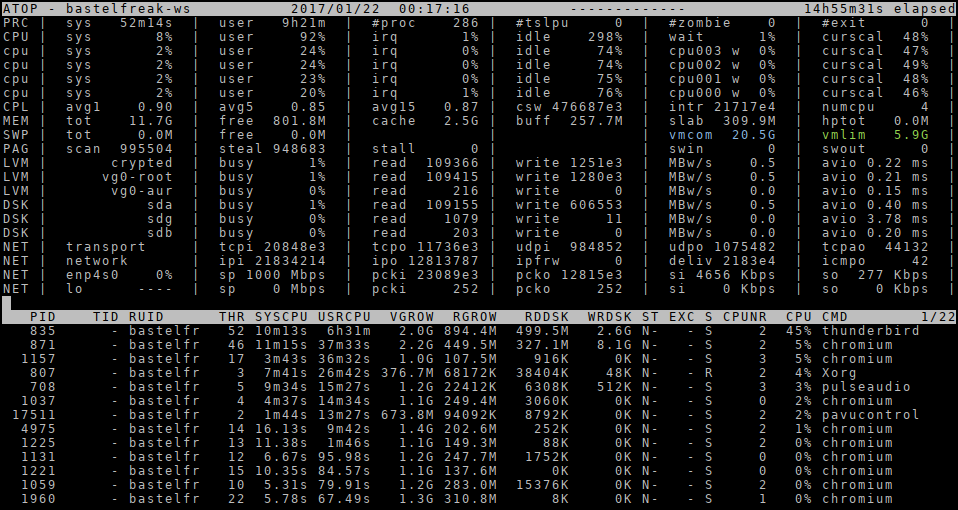
\includegraphics[width=1.0\textwidth]{../figures/atop_1.png}
  \caption{atop mit geringer Systemlast}
\label{figure:atop1}
\end{figure}

\begin{figure}[tbp]
  \centering
  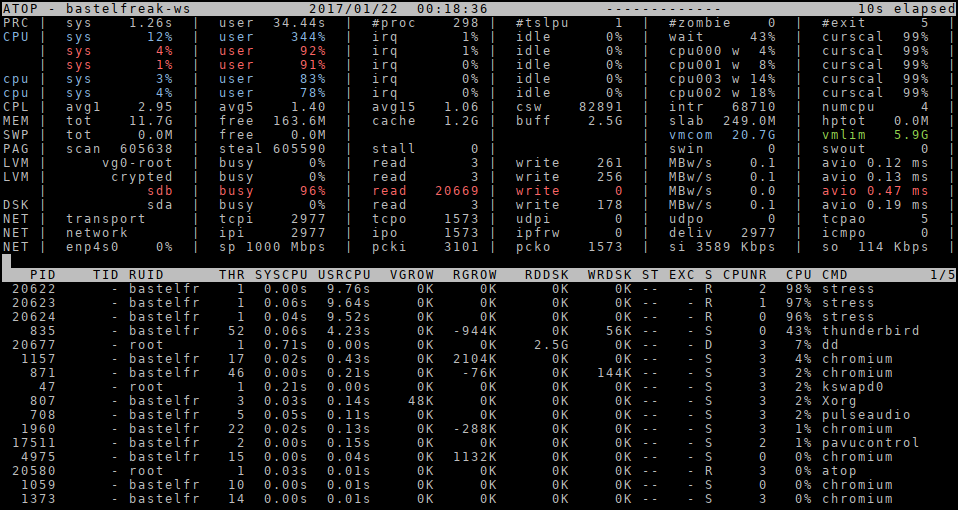
\includegraphics[width=1.0\textwidth]{../figures/atop_2.png}
  \caption{atop mit hoher CPU/Netzwerk Last}
\label{figure:atop2}
\end{figure}

\begin{figure}[tbp]
  \centering
  
\includegraphics[width=1.0\textwidth]{../figures/diamond.png}
  \caption{Offene PRs und Issues im Diamond Projekt am 22.01.2017}
\label{figure:diamond}
\end{figure}

\begin{figure}[tbp]
  \centering
%%  \includesvg[svgpath=../figures/,path=../figures/]{messagebusv1}
  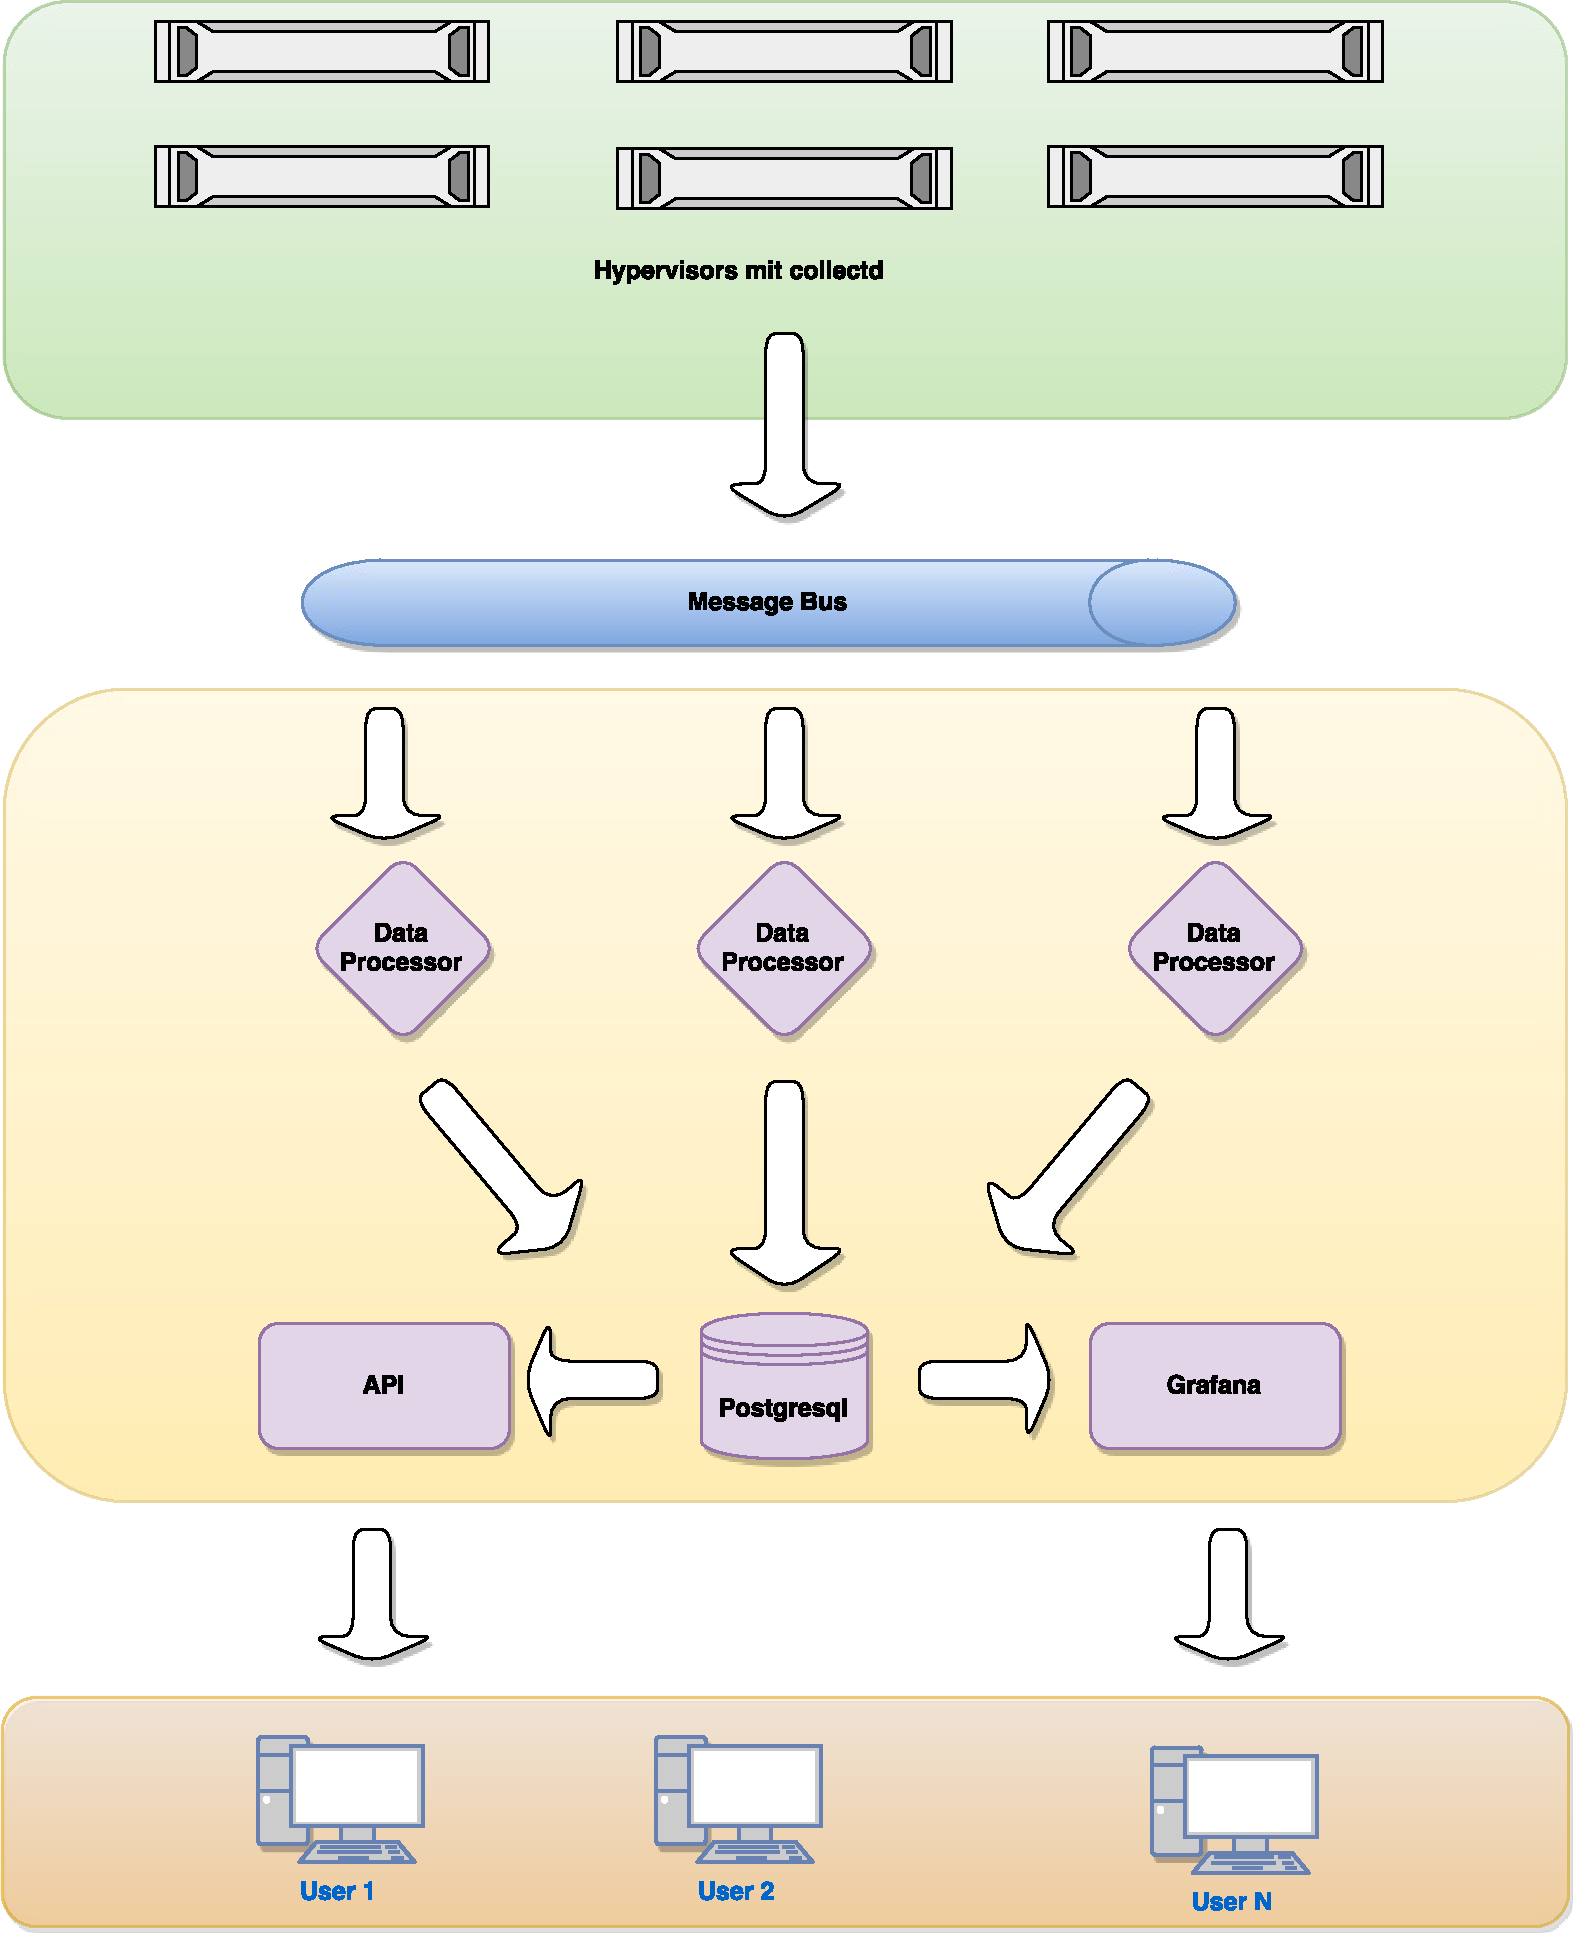
\includegraphics[width=1.0\textwidth]{../figures/messagebusv1_2.pdf}
  \caption{Architekturdraft Version 1}
\label{figure:draft1}
\end{figure}
\begin{figure}[tbp]
  \centering
%%  \includesvg[svgpath=../figures/,path=../figures/]{messagebusv1}
  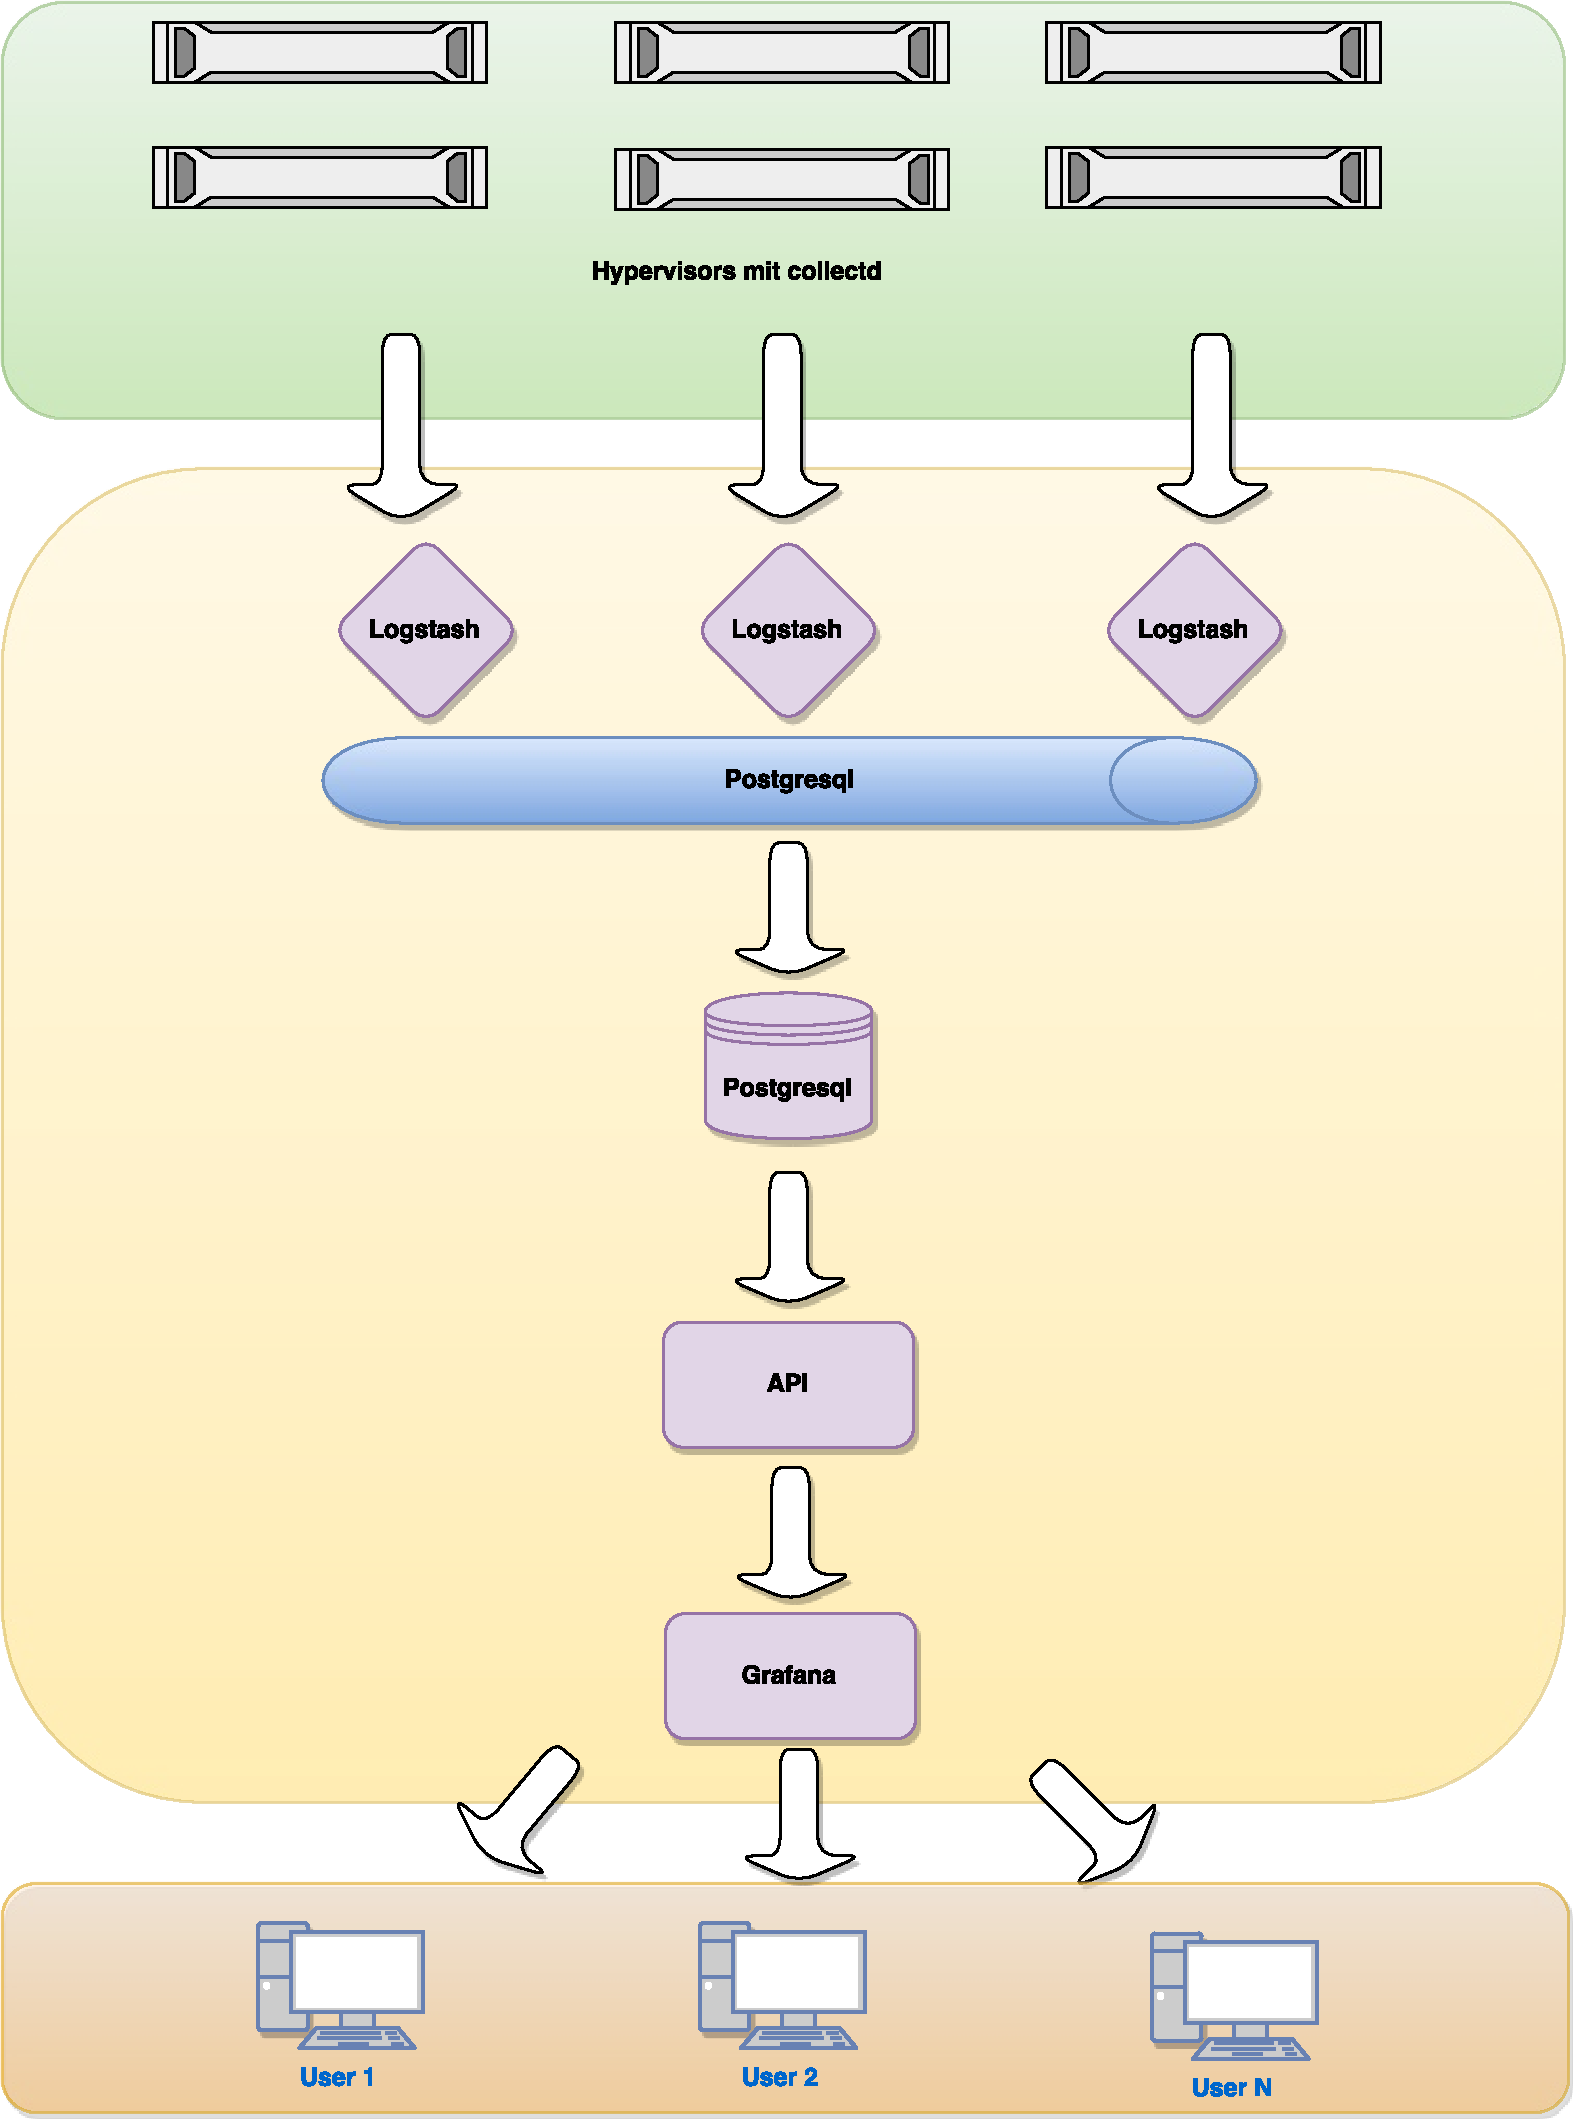
\includegraphics[width=1.0\textwidth]{../figures/messagebusv2_3.pdf}
  \caption{Architekturdraft Version 2}
\label{figure:draft2}
\end{figure}
\FloatBarrier{}

\begin{figure}[tbp]
  \centering
  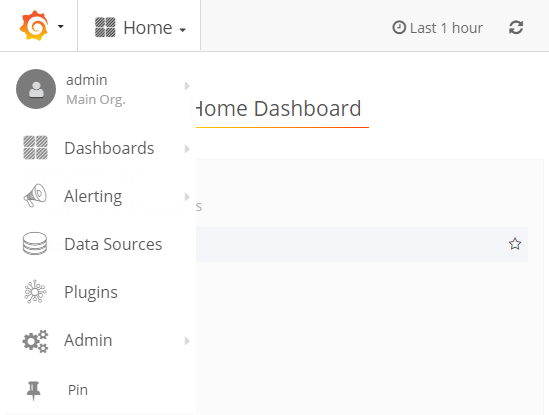
\includegraphics[width=1.0\textwidth]{../figures/grafana_dashboard.png}
  \caption{Grafana Dashboard}
\label{figure:grafana_dashboard}
\end{figure}

\begin{figure}[tbp]
  \centering
  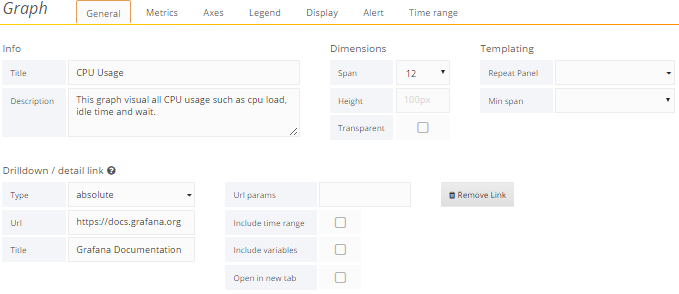
\includegraphics[width=1.0\textwidth]{../figures/grafana_general.png}
  \caption{Grafana Graph Menüpunkt General}
\label{figure:grafana_general}
\end{figure}

\begin{figure}[tbp]
  \centering
  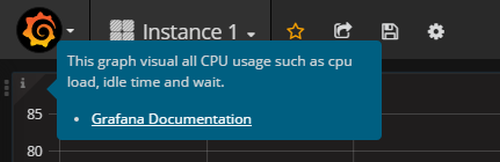
\includegraphics[width=1.0\textwidth]{../figures/grafana_description.png}
  \caption{Grafana Graph Beschreibung}
\label{figure:grafana_description}
\end{figure}

\begin{figure}[tbp]
  \centering
  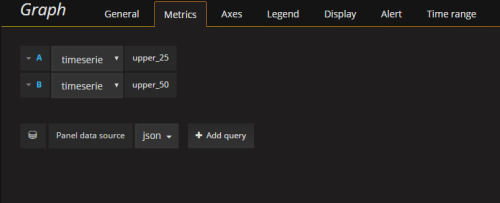
\includegraphics[width=1.0\textwidth]{../figures/grafana_metrics.png}
  \caption{Grafana Graph Metriks}
\label{figure:grafana_metrics}
\end{figure}

\begin{figure}[tbp]
  \centering
  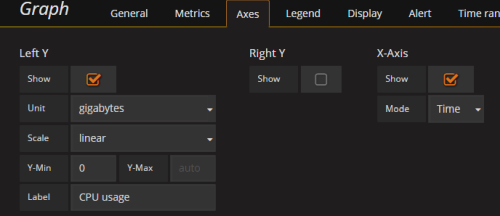
\includegraphics[width=1.0\textwidth]{../figures/grafana_axes.png}
  \caption{Grafana Graph Axen}
\label{figure:grafana_axes}
\end{figure}

\begin{figure}[tbp]
  \centering
  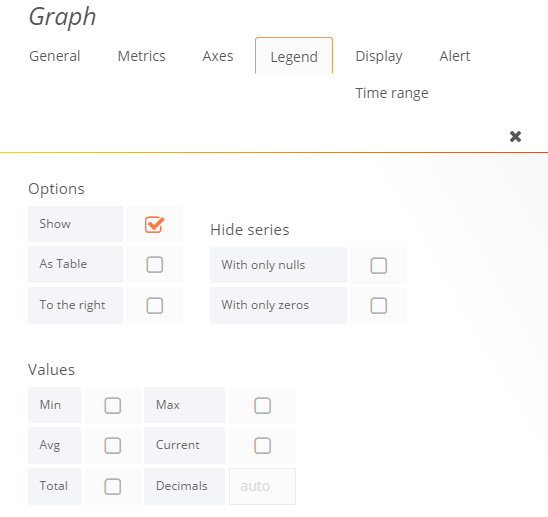
\includegraphics[width=1.0\textwidth]{../figures/grafana_legend.png}
  \caption{Grafana Graph Legende}
\label{figure:grafana_legend}
\end{figure}

\begin{figure}[tbp]
  \centering
  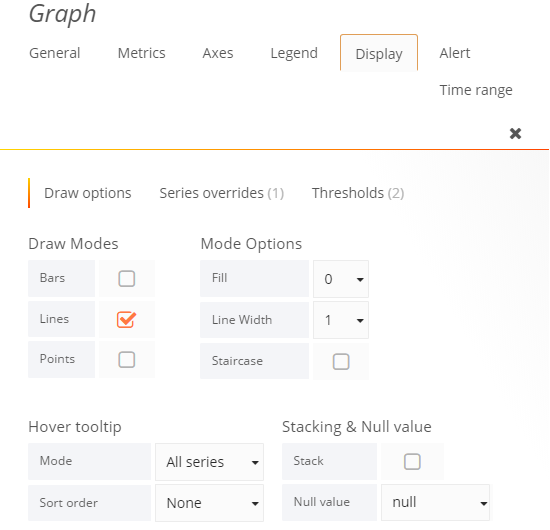
\includegraphics[width=1.0\textwidth]{../figures/grafana_display.png}
  \caption{Grafana Graph Display}
\label{figure:grafana_display}
\end{figure}

\begin{figure}[tbp]
  \centering
  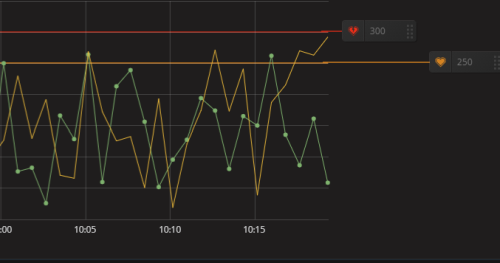
\includegraphics[width=1.0\textwidth]{../figures/grafana_thresholds.png}
  \caption{Grafana Graph Schwellenwert Beispiel}
\label{figure:grafana_thresholds}
\end{figure}

\begin{figure}[tbp]
  \centering
  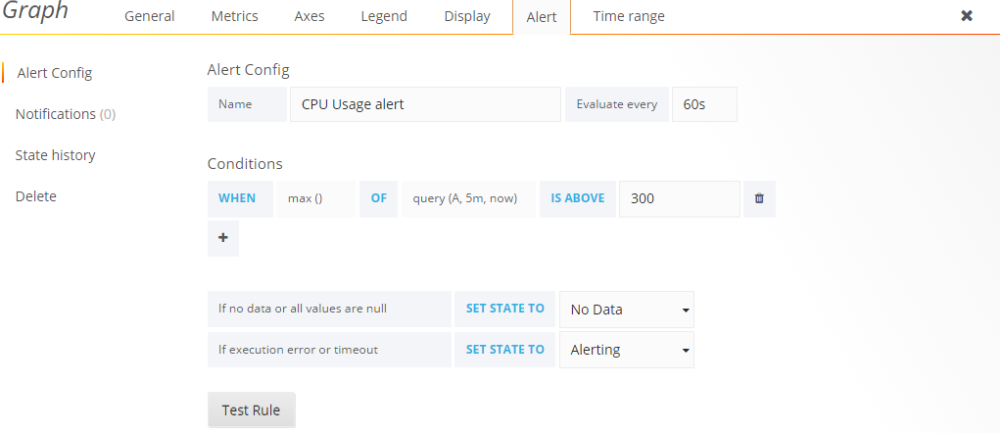
\includegraphics[width=1.0\textwidth]{../figures/grafana_alert.png}
  \caption{Grafana Graph Benachrichtigung}
\label{figure:grafana_alert}
\end{figure}

\begin{figure}[tbp]
  \centering
  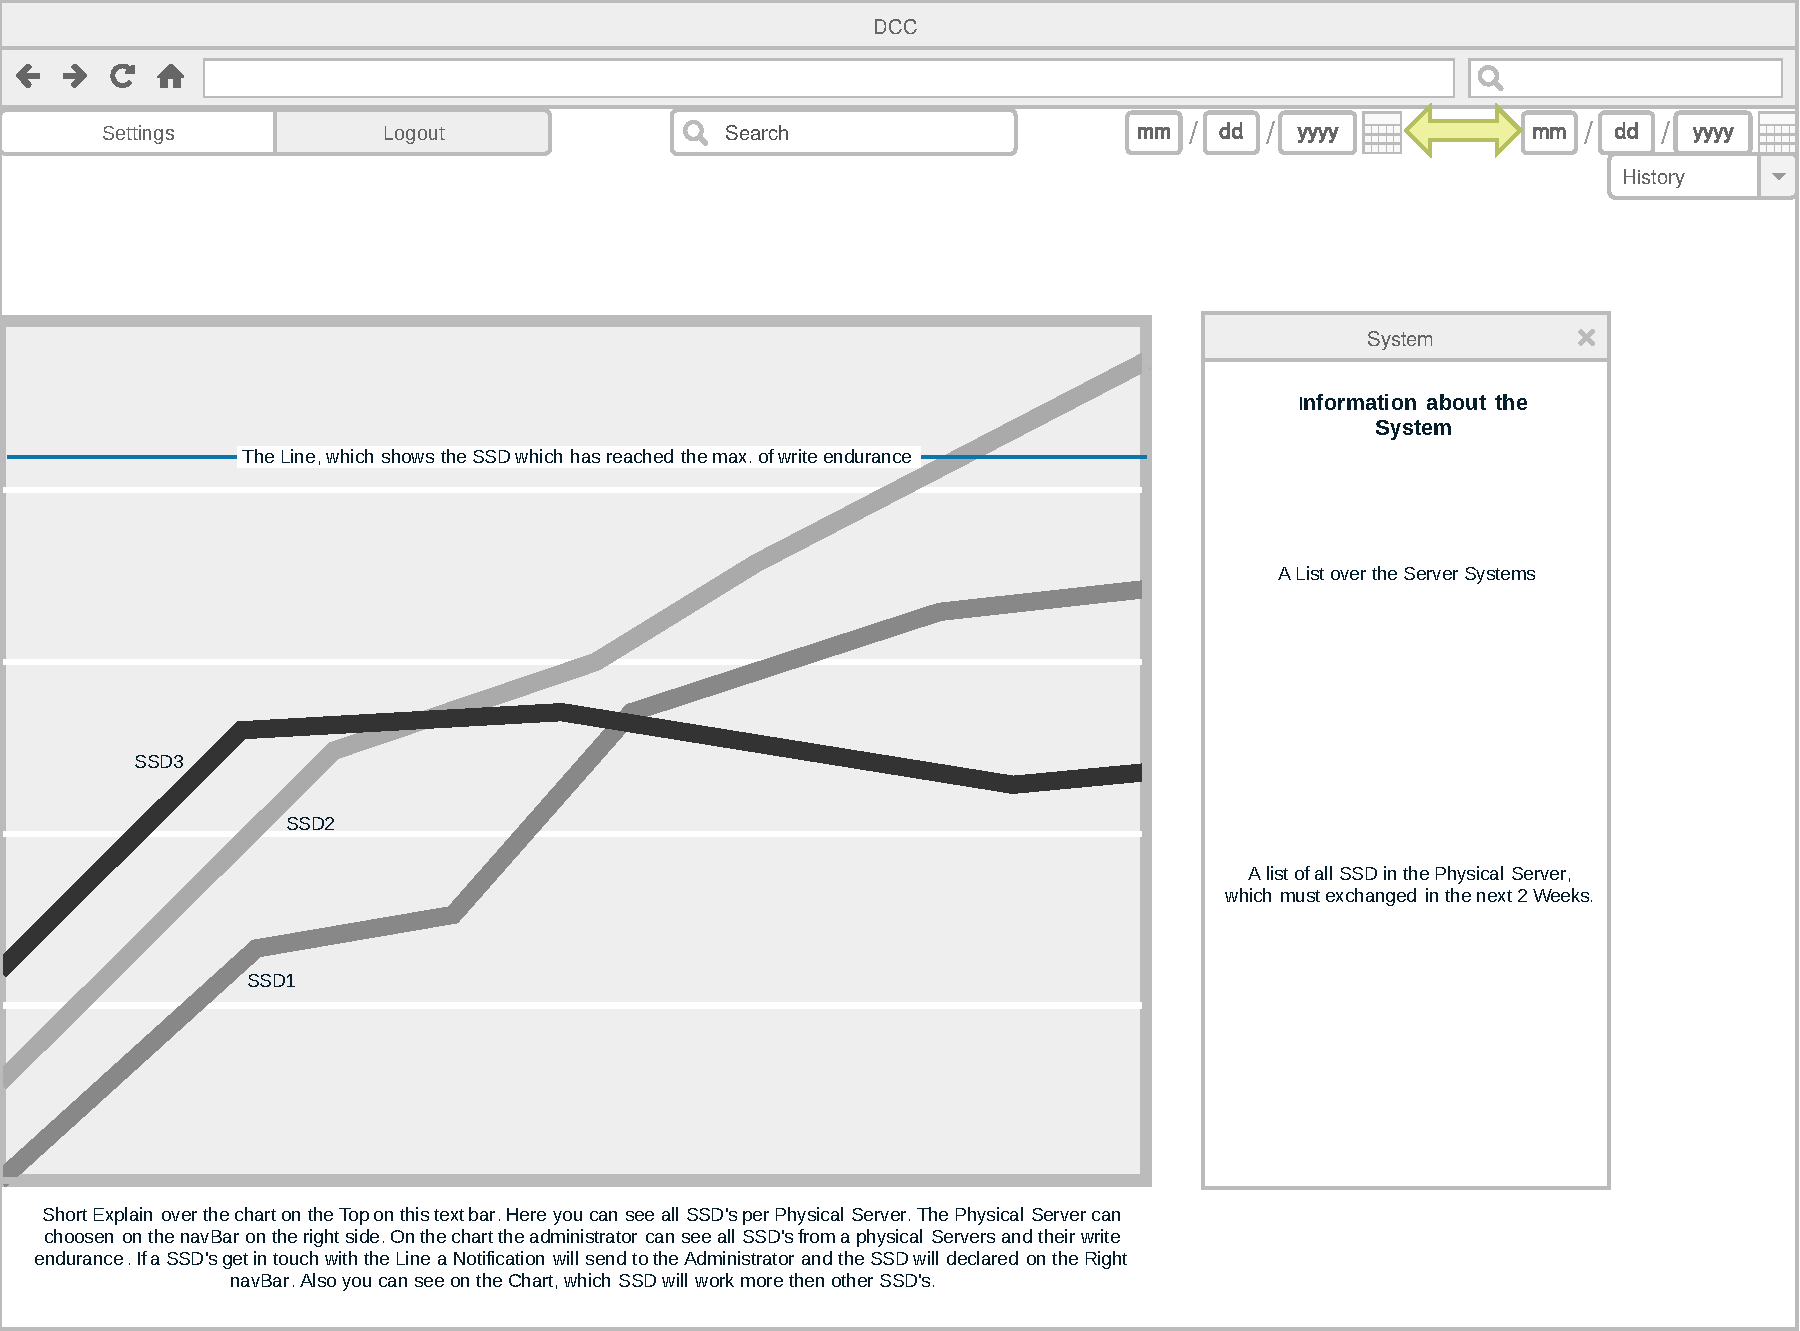
\includegraphics[width=1.0\textwidth]{../figures/ssduserstory-crop.pdf}
  \caption{Wireframe für SSD Userstory}
\label{figure:ssduserstory}
\end{figure}

\begin{figure}[tbp]
  \centering
  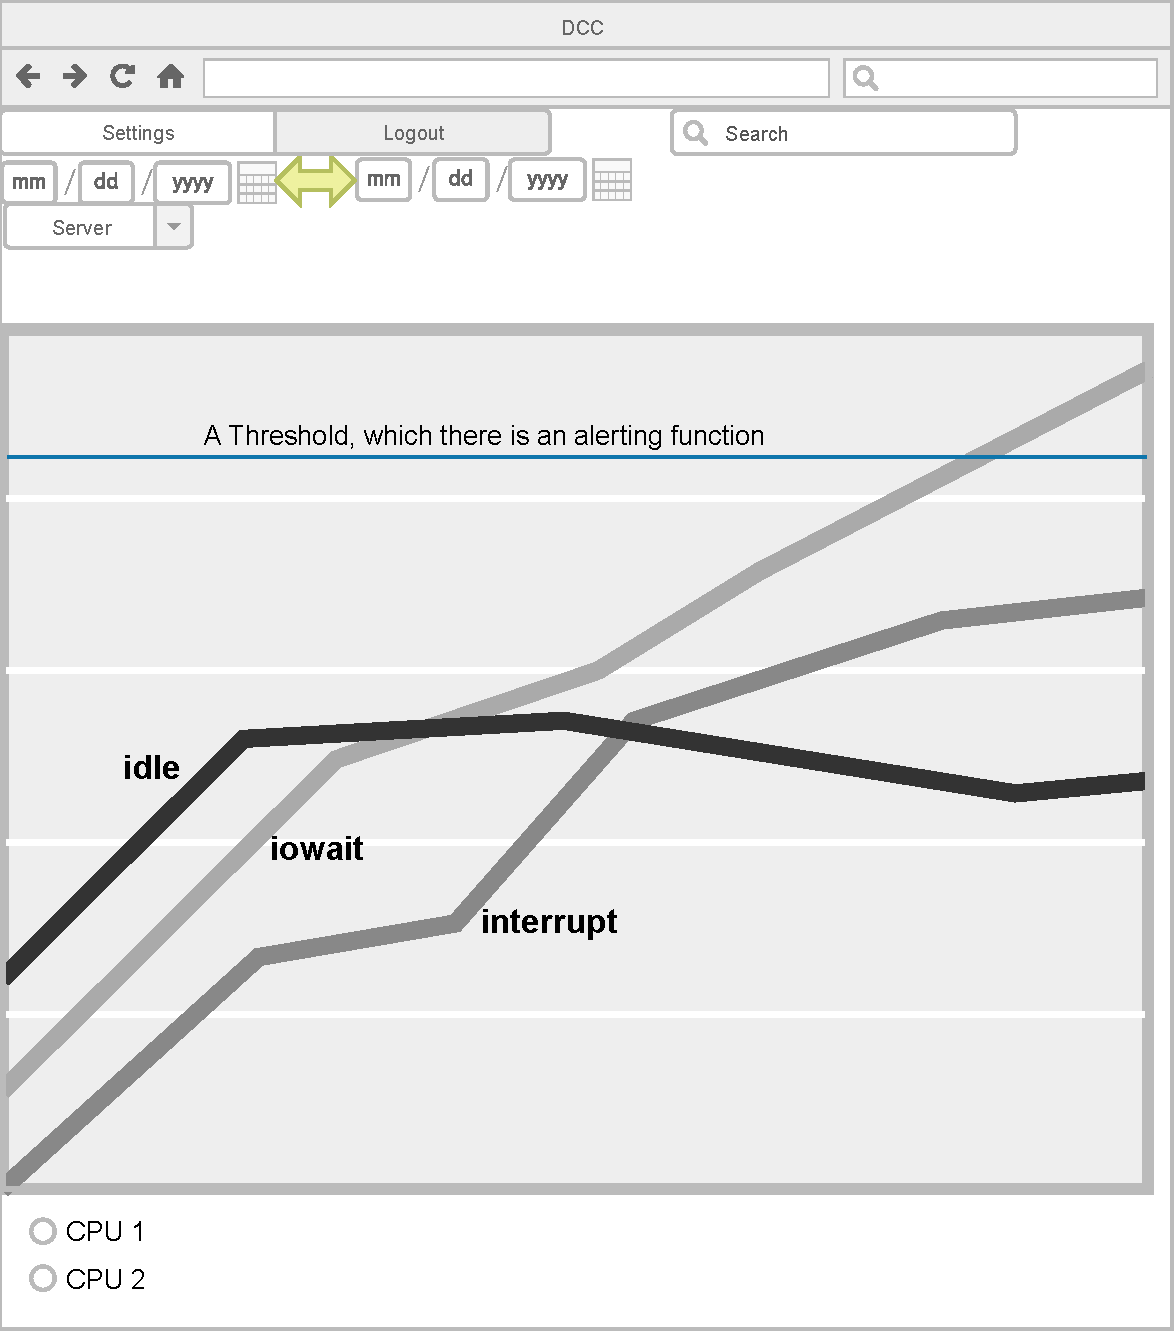
\includegraphics[width=1.0\textwidth]{../figures/cpuuserstory-crop.pdf}
  \caption{Wireframe für CPU Userstory}
\label{figure:cpuuserstory}
\end{figure}

\begin{figure}[tbp]
  \centering
  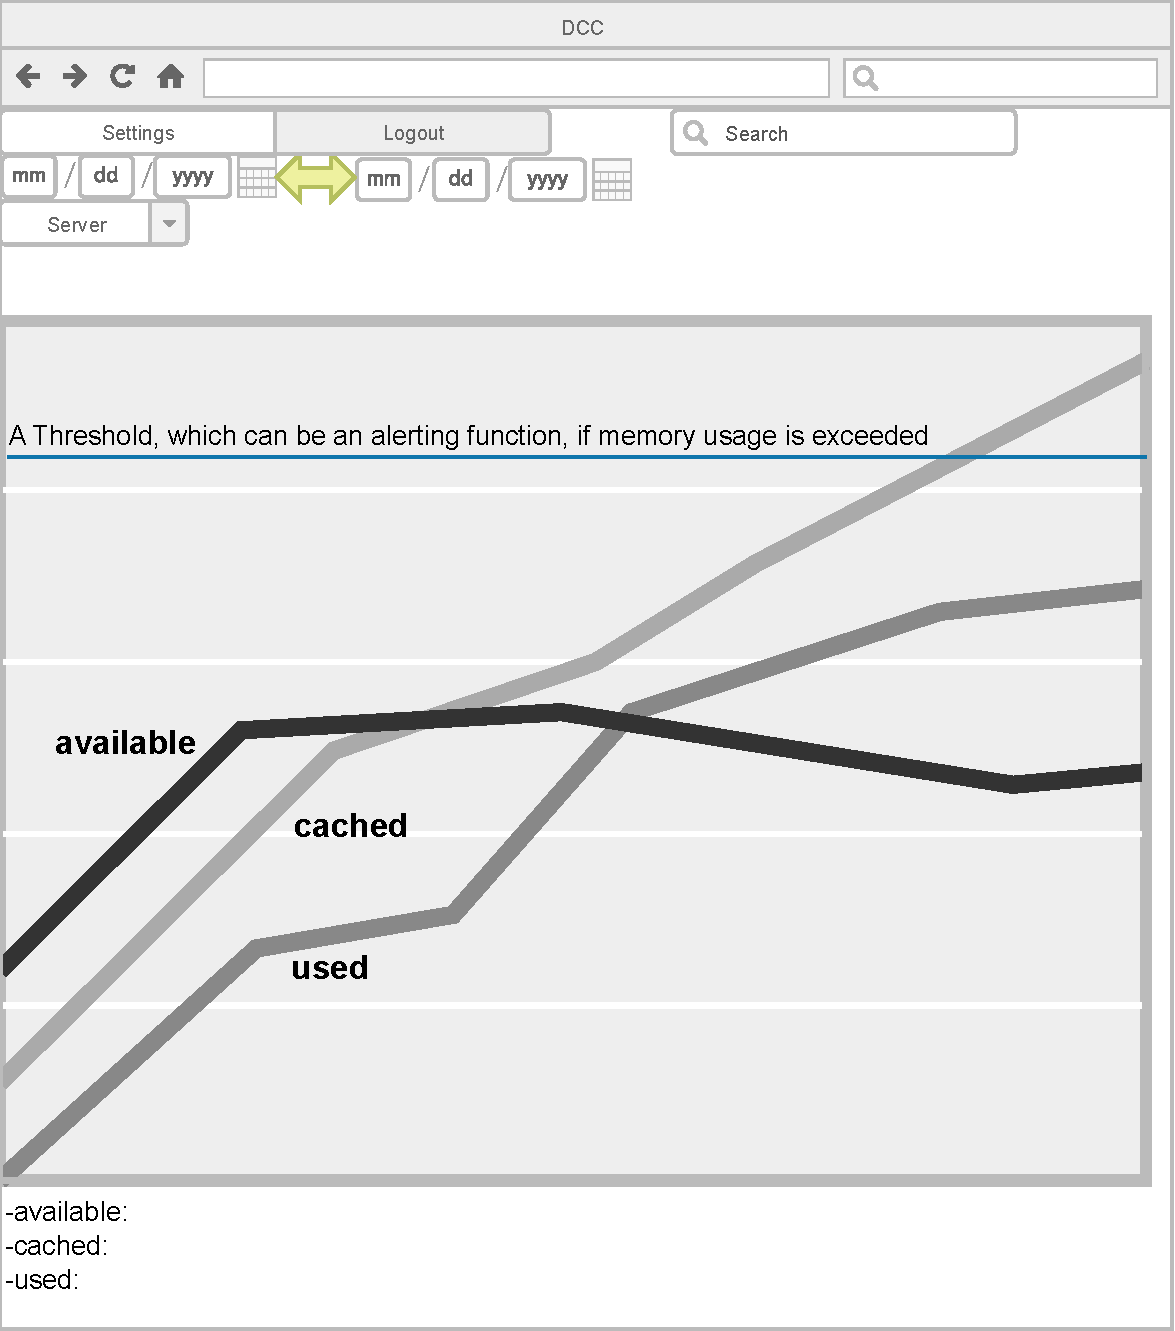
\includegraphics[width=1.0\textwidth]{../figures/memoryuserstory-crop.pdf}
  \caption{Wireframe für Memory Userstory}
\label{figure:memoryuserstory}
\end{figure}

\begin{figure}[tbp]
  \centering
  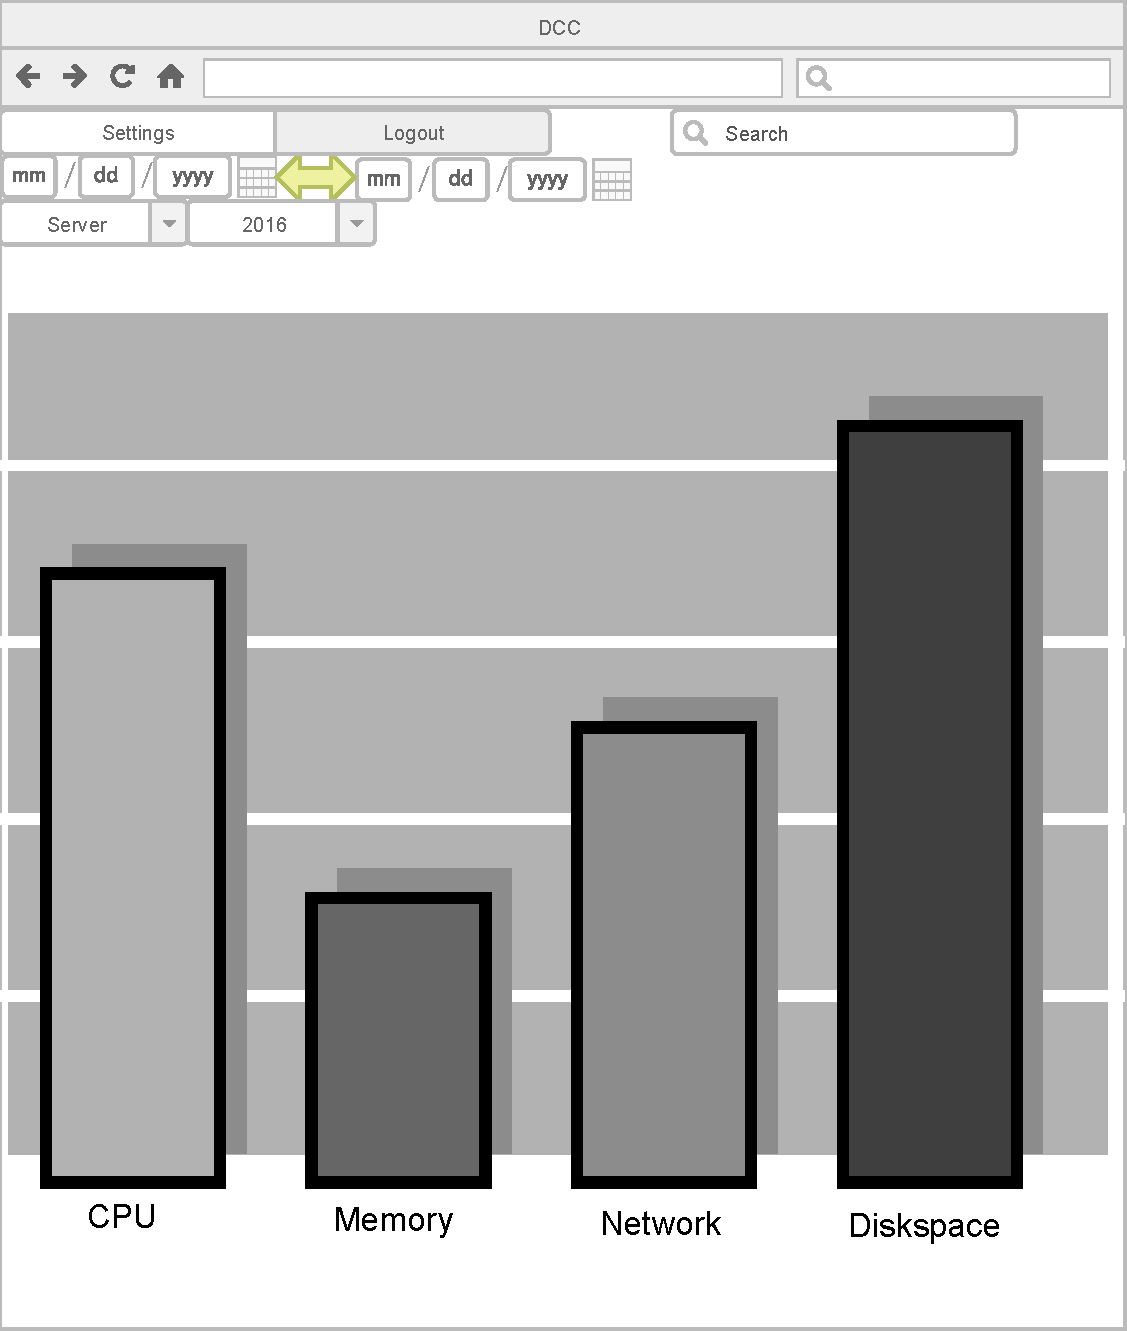
\includegraphics[width=1.0\textwidth]{../figures/timeframeuserstory-crop.pdf}
  \caption{Wireframe für Zeitdefinierte Analyse Userstory}
\label{figure:timeframeuserstory}
\end{figure}

\begin{figure}[tbp]
  \centering
  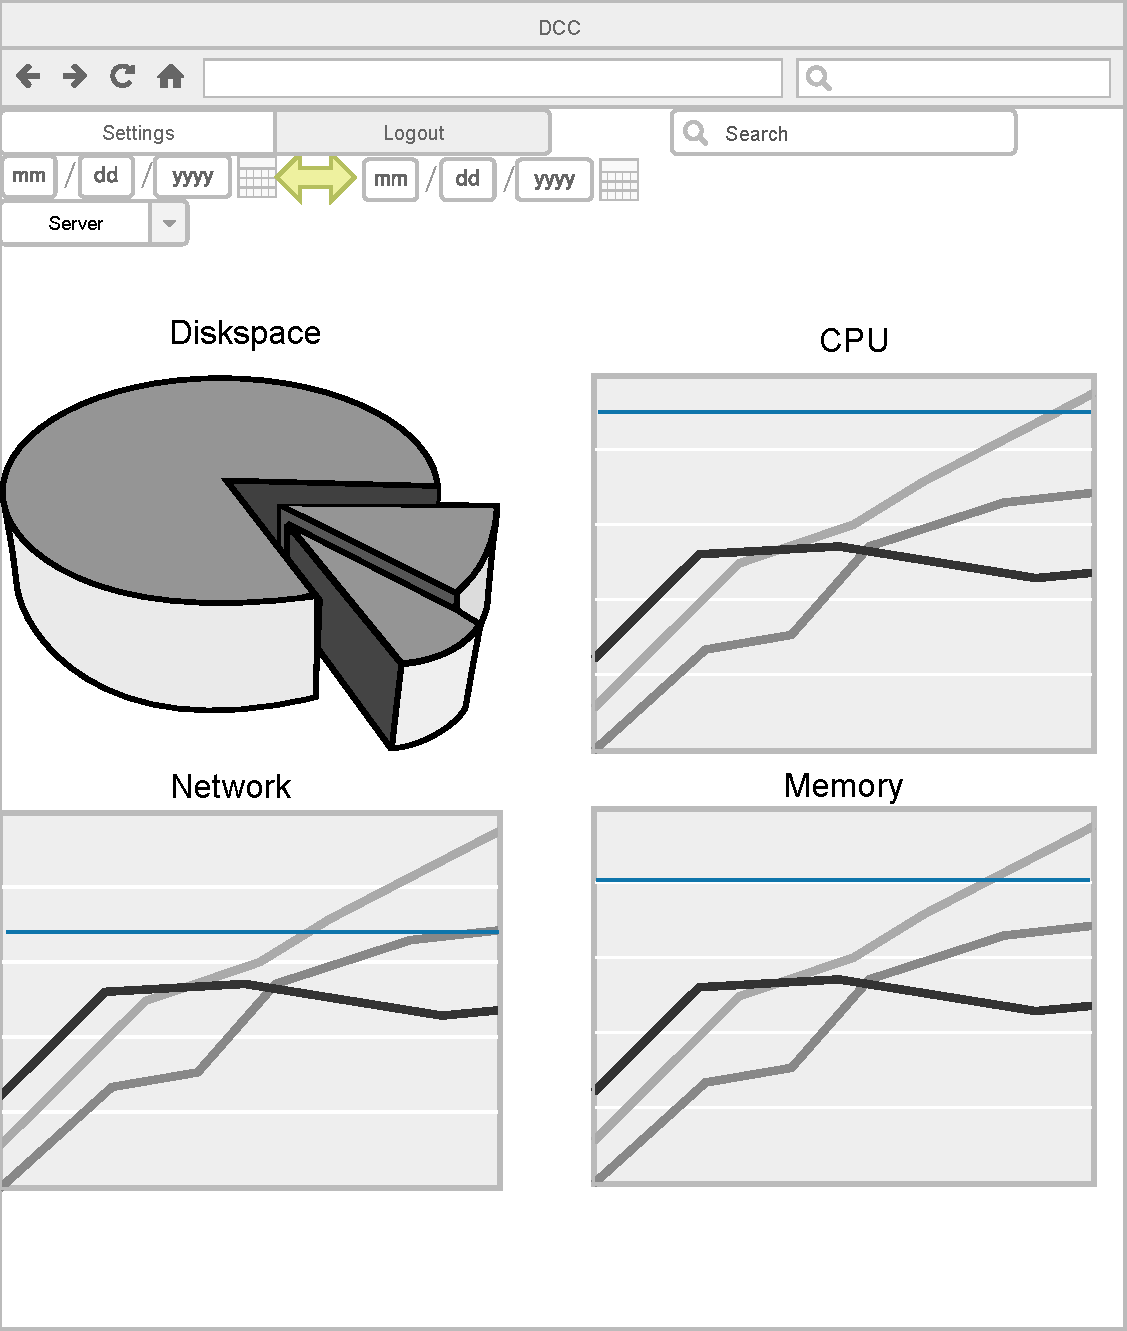
\includegraphics[width=1.0\textwidth]{../figures/uiuserstory-crop.pdf}
  \caption{Wireframe für Weboberfläche Userstory}
\label{figure:uiuserstory}
\end{figure}
